\documentclass{article}

% Language setting
% Replace `english' with e.g. `spanish' to change the document language
\usepackage[english]{babel}

% Set page size and margins
% Replace `letterpaper' with`a4paper' for UK/EU standard size
\usepackage[letterpaper,top=2cm,bottom=2cm,left=3cm,right=3cm,marginparwidth=1.75cm]{geometry}

% Useful packages
\usepackage{amsmath}
\usepackage{graphicx}
\usepackage[colorlinks=true, allcolors=blue]{hyperref}

\title{Travlr ID: Decentralising Travel Data Management with DePIN and AI agents}
\author{\href{https://www.dipankar.name}{\hspace{1mm}Dipankar Sarkar} \\
  \texttt{dipankar@travlrid.com} \\
        \and
	Gee Mann \\
	%% Address \\
	\texttt{gee@travlrid.com} \\
	%% \And
	%% Coauthor \\
	%% Affiliation \\
	%% Address \\
	%% \texttt{email} \\
	%% \And
	%% Coauthor \\
	%% Affiliation \\
	%% Address \\
	%% \texttt{email} \\
 }
\begin{document}
\maketitle

\begin{abstract}
This whitepaper introduces Travlr ID, a groundbreaking solution designed to address data challenges in the travel industry. Using blockchain technology and artificial intelligence, Travlr ID proposes a Decentralized Physical Infrastructure Network (DePIN) that transforms travel data management. Provides consumers with a digital vault to securely store and delegate access to their data. Service providers also benefit from this solution, gaining efficient access to necessary data, reducing redundancy, and improving service personalisation. DePIN, combined with decentralized AI agents, improves data usage, streamlines operations, and delivers personalized travel experiences. The paper discusses the technology behind Travlr ID, its practical implementation, potential benefits, and future scalability. With its forward-thinking approach, Travlr ID aims to revolutionize the travel industry, offering a future where data management is secure, efficient, and respects user privacy.
\end{abstract}

\pagebreak

\tableofcontents

\pagebreak

\section{Introduction}

The travel industry is a vast interconnected ecosystem of travelers and service providers, ranging from airlines to hotels, from restaurants to event organizers. Each entity in this network needs access to a variety of consumer data to optimally function and provide personalized, efficient, and exceptional services to travelers. However, the current data sharing model is highly fragmented and often exposes travelers to vulnerabilities.

Each journey a traveler undertakes begins with the planning stage, which involves an exchange of information. This information is shared with various travel service providers who further relay this data to various other entities involved in arranging the journey. It is not uncommon for the traveler to repetitively share and verify personal data, a practice that not only proves tiresome to the traveller but poses a significant risk to their privacy. Moreover, this vast amount of valuable generated data often remains scattered, under-utilized, or locked behind regulatory and privacy concerns.

Currently, the travel data supply chain involves countless intermediaries that collect, transfer and store personal consumer data. This legacy infrastructure was not designed to handle the sheer volume, variety, and velocity of the data currently generated by travelers, and is thus riddled with inefficiencies, redundancies, and is prone to data breaches.

Although advances in technology offer possibilities for optimizing the data supply chain, it is becoming increasingly clear that more than an upgrade, a paradigm shift is necessary. The privacy of users is increasingly being recognized as a fundamental right, creating additional legal, ethical, and practical obstacles for the current state of data handling in the travel industry. Moreover, as a traveler's journey becomes more digitized, the challenge of managing and protecting an ever-growing volume of sensitive data increases.

 In this paper we introduce Travlr ID, a cutting-edge solution that aims to solve the conundrum of data challenges in the travel industry through the use of decentralized technology. Our proposed model rethinks the way data is collected, stored, and shared, placing control back into the hands of consumers while providing efficient and effective solutions for service providers. As we dive deeper into this whitepaper, we will explore the structural design and functional benefits of Travlr ID and explore how it strives to revolutionize the travel data supply chain by harnessing cutting-edge techniques such as blockchain and Artificial Intelligence (AI).

\pagebreak

\section{Travel Industry - Data Supply Chain}

In this digital age, almost every aspect of travel - be it the booking of flights, car rentals, hotels, adventures, or even dining experiences - depends heavily on data exchange. Travelers provide their personal and trip details, which are then processed by various travel service providers to create customized experiences. However, this flow of data, while necessary, has far-reaching implications related to privacy, security, and efficiency.

The data supply chain in the travel industry is convoluted, complex, and intricate. At every stage of a traveler’s journey – from initial reservation to final check-out – a multitude of entities collect, transmit and accumulate personal data. The global tourism industry, which accounted for 10.4\% of the world's GDP in 2019, involves significant data exchange.

Unfortunately, the immense complexity of this data supply chain presents a host of challenges for both consumers and service providers. While service providers face the challenge of efficiently handling and leveraging these data, consumers are increasingly concerned about their privacy and security.

Lets look at each of these challenges individually. 

\subsection{Data Fragmentation}

With each new reservation, flight check-in, or hotel stay, multiple data touchpoints are created. As it stands, the various entities involved, ranging from airlines to hotel chains, and from travel agencies to tourism attractions, operate in silos hoarding the data they generate. This fragmentation prevents a seamless and integrated customer experience while posing security risks, as each entity must protect the data from breaches.

Burgeoning technologies such as machine learning, artificial intelligence, and predictive analytics have great potential to revolutionize the travel industry, but the siloed nature of the data prevents these tools from reaching their full potential. Moreover, repeated collection and verification of data at each step is both a headache for the customer and an operational inefficiency.

\subsection{Privacy Challenges}

Currently, there is an apparent gap in the travel data management landscape. The industry lacks a centralized, secure and efficient data sharing protocol, which prevents the optimization of services and the smooth transition of services from one provider to another. Consumers also lack the ability to control who accesses their data and for what purpose, raising privacy concerns.

Several data breaches over the years have highlighted the vulnerability of existing systems. Therefore, the need for a paradigm shift in data management in the travel industry cannot be overstressed. Next-generation solutions need to revolve around improved data security, improved interoperability, and giving control back to consumers.

\begin{table}[ht]
\centering
\begin{tabular}{|p{4cm}|p{5cm}|p{6cm}|}
\hline
\textbf{Challenge} & \textbf{Today} & \textbf{Blockchain and AI-Based Future} \\
\hline
\textbf{Data Fragmentation} & 
Data is stored in silos, hindering integration and insights. & 
Decentralized network allows seamless data sharing, enabling complete insights. \\
\hline
\textbf{Privacy
Challenges} & 
Consumers lack control over data access, raising privacy concerns. & 
Consumers have full control over data using private keys and zero-knowledge proofs. \\
\hline
\textbf{Security Risks} & 
Frequent data breaches highlight system vulnerabilities. & 
Blockchain reduces breach risks with cryptographic principles and decentralization. \\
\hline
\textbf{Regulatory Compliance} & 
Complex compliance with regulations, risking severe penalties. & 
Immutable ledger and consumer-controlled sharing facilitate easier compliance. \\
\hline
\textbf{Operational Inefficiencies} & 
Repeated data collection creates redundancy and inefficiencies. & 
Real-time, Decentralized data access and AI streamline operations, enhancing experience. \\
\hline
\textbf{Under-utilization of Technology} & 
Siloed data prevents AI and analytics from optimizing services. & 
Integrated data on a decentralized network enhances AI and analytics potential. \\
\hline
\end{tabular}
\caption{Comparison of Data Supply Chain Challenges: Today vs. Blockchain and AI-Based Future}
\label{table:comparison}
\end{table}


\subsection{Need for Blockchain}

This section takes a deep dive into the innovative world of blockchain technology, explaining its concepts, functionalities, and potential benefits it could bring to the travel industry. Highlighting emerging concepts such as Zero-knowledge proofs, we aim to elaborate on how blockchain could pave the way for a new era in data management.

\subsubsection{Digital Ledger}

Simply put, a blockchain is a digital ledger, a secure chain of blocks that stores data across multiple systems, ensuring decentralization and preventing any single entity from having sole authority over data. Every block is secured using cryptographic principles, ensuring data is extremely difficult to alter or manipulate once written into the chain.

Newer technologies like Zero-knowledge proofs enhance this security even further. Zero-knowledge proofs allow one party (the prover) to prove to another party (the verifier) that a given statement is true, without conveying any additional information apart from the fact that the statement is indeed true. This strengthens privacy, as no specific details need to be revealed during the verification of transactions.

\subsubsection{Benefits \& Advantages}

Known for its decentralization, transparency, and security, blockchain technology has garnered immense interest from various industries, and rightfully so. It ensures data integrity, eliminates intermediaries, reduces the potential for fraud, and promises enhanced privacy through techniques like Zero-knowledge proofs. 

As a decentralized technology, blockchain forms a network of peer-to-peer transactions. Its transparency fosters trust among users, as all transaction data (excluding private details protected by zero-knowledge proofs or similar protocols) is visible to every participant of the chain.

\subsubsection{Travel industry applications}

Blockchain offers a multitude of benefits in the travel sector, notably improving efficiency, security, and consumer trust. Airlines can use it to manage frequent flyer points and baggage tracking. Hotels could use it for room booking and travel agencies for maintaining secure and transparent ticketing.

By enabling permissioned data sharing (like via Travlr ID), customer verification becomes smooth, yet secure. Furthermore, the implementation of Zero-knowledge proofs can help demonstrate the validity of a traveler's credentials without having to expose any sensitive personal information.

The potential extends to overcoming regulatory hurdles like GDPR, as blockchain technology allows for a system where customers have the power to decide who can access their data, adding another layer of data protection and privacy.

\subsection{Summary}

Today, the data in their current form remain in \textbf{disjoint silos} within the industry, hindering the ability to gain complete insight at the various stages of the traveler’s journey. Each step often requires separate data submission and verification, leading to redundancy and inefficiencies. The problems arising from these fragmented systems can inevitably erode the customer experience.

\textbf{Security} represents another significant challenge, as data breaches become increasingly common in the global digital landscape. In 2019 alone, Marriott International, one of the largest hotel chains in the world, declared that 383 million guest records were compromised, including 5 million passport numbers.

In addition, the problem is exacerbated when considering the multitude of local, national, and international \textbf{regulations} governing the use, storage, and transfer of personal data. Stringent acts such as the European General Data Protection Regulation (GDPR) require solid data handling infrastructures and practices, penalizing companies up to 4\% of their global revenue for violations.

The existing data management approach in the travel sector is plagued by fragmentation, under-use, security risks, and legal obstacles. These issues collectively underscore the critical and immediate need for an all-encompassing solution that can simplify the travel data supply chain while protecting data security, confidentiality, and adherence to regulations.

\newpage

\section{Travlr ID Protocol}

Travlr ID brings an exciting and revolutionary solution to the travel industry's data challenges. An intricate architecture based on blockchain technology and state-of-the-art data security practices is at the core of this initiative. This chapter unfolds the distinct segments of this architecture and explores how each one contributes towards realizing the vision of Travlr ID.

\subsection{Vision \& Goals}

In the face of increasing data management challenges in the travel industry, Travlr ID proposes a groundbreaking solution that uses the potential of blockchain technology, decentralization, and artificial intelligence.

Travlr ID aims to revolutionize the travel industry by allowing both consumers and service providers to have a more secure, efficient, and decentralized means of data sharing. Using a unique blockchain-based framework, the aim is to establish a system where data can be stored in a blockchain vault, managed by the consumer, and shared only with their permission.

Various service providers, including hotels, airlines, and restaurants, can then interact with this vault, reducing the need for constant re-verification and eliminating data redundancy. In addition, it provides space for decentralized AI agents to interact with this data (with the consumer's consent), finding deals, identifying events, and personalizing travel experiences. 

\paragraph{Vision} Travlr ID's vision is to pioneer a new era in the travel industry where the power of personal data is given back to the customer, strengthening the trust and transparency in data handling. It aims to create a universal data sharing model that is not only robust, transparent, and secure but also adheres to stringent data privacy regulations. 

\paragraph{Goal} Our goal is to foster a digitally evolving ecosystem where technology facilitates seamless journeys, data drives customer satisfaction, and privacy is a priority.

\begin{itemize}
    \item \textbf{Consumer Empowerment}: To provide travelers with a tool that gives them full control over their data and the freedom to share it as per their convenience and needs.
    \item \textbf{Data Security}: Ensuring all personal data remain secure with state-of-the-art encryption standards and are accessed only upon consumer's permission.
    \item \textbf{Streamlined Industry Experience}: Helping industry partners assimilate and use customer data efficiently, thus improving their service and ultimately increasing their growth.
    \item \textbf{Regulatory Compliance}: Adherence to international data protection standards and ensuring proactive compliance with rules such as GDPR.
    \item \textbf{Scalability}: Ensuring the framework can not only work across multiple chains but can also keep the transaction and storage costs feasible.
    \item \textbf{Adoption of Emerging Technologies}: Continued pursuit of emerging technologies like decentralized AI to augment the existing framework and deliver ever-improving customer experiences.
\end{itemize}

\subsection{Key Components}

\subsubsection{Consumer Vaults}

A fundamental part of the Travlr ID architecture is the Consumer Vaults. It acts as a digital locker, where consumers can securely store all their personal and travel-related data. Blockchain technology's decentralized nature ensures that the control of these data lies solely with the consumer.

What sets the Travlr ID’s vault apart is ease and control. Using their private keys, consumers decide what information is shared and with whom, ensuring complete control over their personal data. Advanced features like Zero-knowledge proofs can be incorporated, allowing verification of credentials without sharing the actual information.

This not only personalizes their experience, but significantly reduces the need for re-verification at every stage of the travel process, thereby saving time and improving efficiency.

\subsubsection{Service Provider Vaults}

\begin{figure}[h]
    \centering
    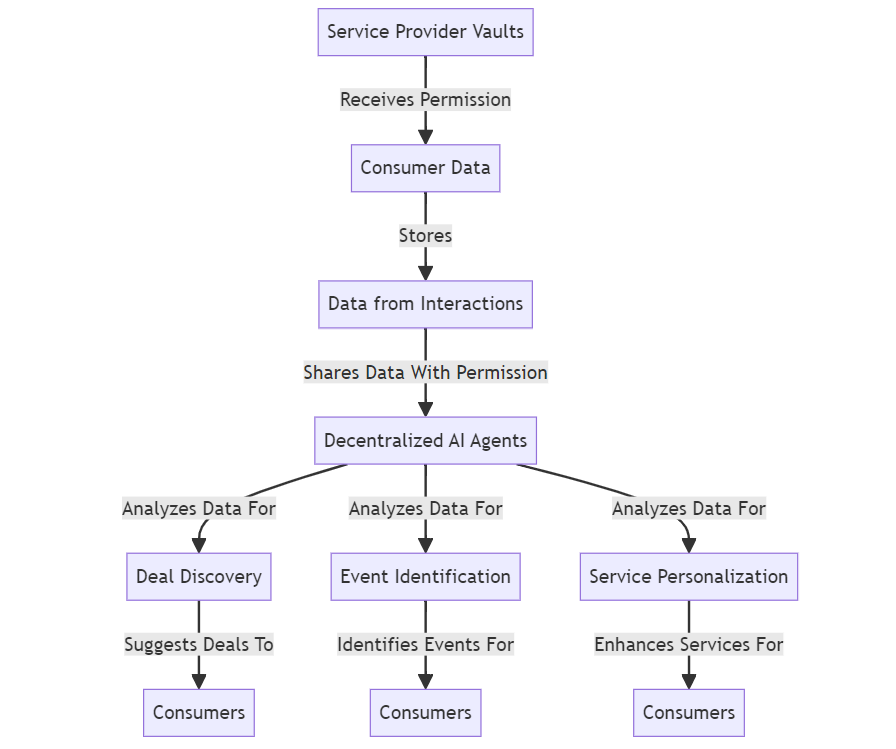
\includegraphics[width=0.6\linewidth]{travlr_diagram_5.png}
    \caption{Service provider vaults}
    \label{fig:enter-label}
\end{figure}

To complete the data-sharing cycle, service providers, such as hotels, airlines, and car rental agencies, can also run their vaults. These vaults can interact with the consumers' vaults and collect necessary data, post receiving permissions.

The adoption of this vault system by service providers ensures a streamlined and efficient data collection and usage process. It negates the need for data reentry, verification at every stage, providing seamless services and a more personalized experience for the traveler.

The service provider vaults can also collect and store data generated during the interactions with the customers. With consumer permission, this information can be used to optimize services and offerings, reinventing the way they interact with and understand their customers.

\subsubsection{Decentralised AI Agents}

Using the power of artificial intelligence, Travlr ID aims to increase the efficiency and personalization of the travel experience. Our Decentralized AI Agents interact with both the consumer and service provider vaults. Consumers and service providers grant permission to these AI agents to use data as needed for deal discovery, event identification, and service personalisation.

The AI agents, while processing large chunks of data, adhere strictly to privacy guidelines and blockchain's secure framework. They can help from the planning phase of a trip, suggesting itinerary based on past travel patterns, through to tracking flight schedules in real time and suggesting adjustments as necessary. 

\subsection{Network Infrastructure}

The development of the Travlr ID ecosystem is a complex endeavor. It requires the creation of a secure and scalable decentralized network infrastructure capable of supporting the high-throughput needs of the contemporary travel industry, while also adhering to the standards of privacy and security.

\subsubsection{Data nodes - Service providers}

The nodes form the backbone of any blockchain-based system. They are the individual parts of the larger data structure that validate and relay transactions. In the Travlr ID ecosystem, these nodes will be primarily deployed and managed by the consortium of travel service providers. These nodes will generate income for the service providers and contribute towards the value of the network. 

Every service provider, such as hotels and airlines, can run their own on-premises nodes. These nodes collect and store the data generated by consumers when they interact with these service providers. The data stored in these nodes are secured and can be shared only when the consumer delegates access to another entity on the network.

This approach has several advantages. It ends the practice of transferring large amounts of data over the network, reducing network load. It also gives service providers a better opportunity to manage and monetize their customer data. 

By running an on-premises node, the service provider also becomes a participant in the Travlr ID network, contributing to the overall stability and security of the platform. It is also worth noting that although these nodes are deployed by individual service providers, they follow strict data management and security protocols dictated by the Travlr ID architecture.

The Travlr ID network's on-prem nodes perform the dual role - they ensure swift and safe consumer interactions at the service provider end while strengthening the overall Travlr ID ecosystem.


\begin{figure}[h]
    \centering
    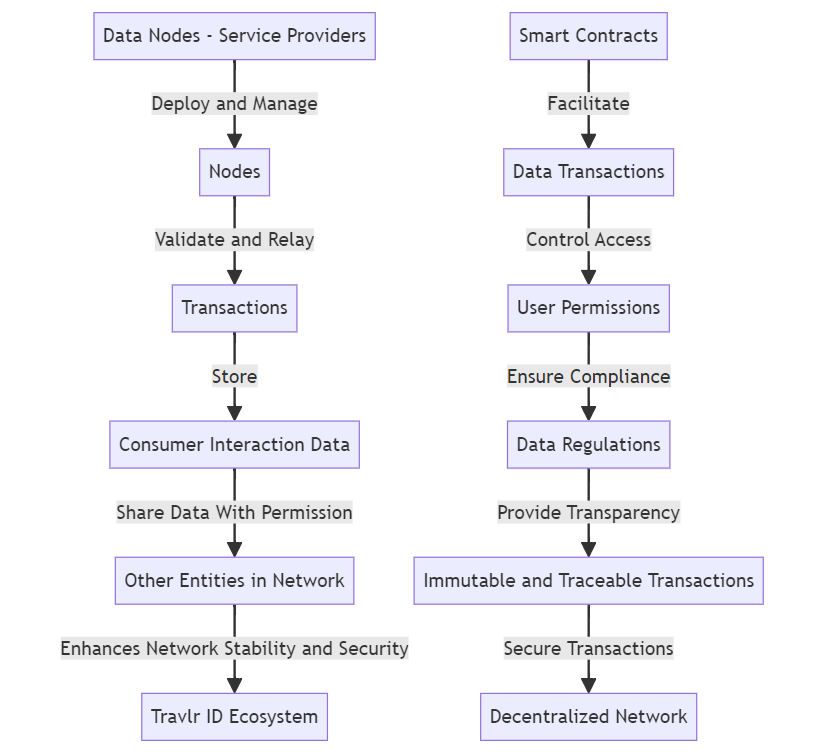
\includegraphics[width=0.6\linewidth]{travlr_diagram_6.png}
    \caption{Service provider \& Smart contracts}
    \label{fig:enter-label}
\end{figure}


\subsubsection{Smart contracts}

At the heart of the Travlr ID blockchain platform is its primary smart contract. A smart contract is a self-executing contract in which the terms of the agreement are written in code. They are a crucial component in ensuring the immutability, security, and trustless nature of the platform.

The primary smart contract in Travlr ID acts as the protocol for the exchange of data between consumer vaults and service provider vaults. Establishes the rules for data control, access, validation, and the level of disclosure depending on user permissions. This smart contract codifies the "rules of engagement" when interacting with a user's vault, ensuring all transactions comply with these rules.

Given the varying nature of different travel service providers, the smart contract is designed with flexibility to accommodate different types of data and interactions. At each step of integrating a service provider into the Travlr ID network, smart contracts can be extended or customized to handle the unique interactions and data requirements for that provider.

This smart contract is being deployed on an EVM blockchain, serving as the foundational layer for the decentralized network. Ensure that all data transactions are secure, private, and transparent.

In essence, the primary smart contract is the driving force that facilitates and governs the secure sharing and transaction of data on the Travlr ID platform. It ensures that the principles of blockchain, such as decentralization and security, while integrating advanced techniques like zero-knowledge proofs, are met in a proper way.

\subsection{Protocol Use-Cases}

We explore two illustrative examples that demonstrate the tangible benefits and potential of Travlr ID for both consumers and service providers.

\subsubsection{Consumer Perspective}

Meet Alex, an avid traveler who frequently embarks on exploratory journeys around the world. Using Travlr ID, Alex can easily and securely plan his upcoming trip to Spain. He starts by entering his travel plans and personal preferences into his Travlr ID vault.

With his permission, a Decentralized AI agent scans and processes his data. It suggests a personalized travel itinerary for Alex based on his preferences and previous travel patterns. The AI Agent also identifies the best flights for his travel dates, recommends hotels meeting his comfort level and budget, and even curates a diverse list of local experiences that align with Alex's interest in art and cuisine.

Once Alex validates and selects an itinerary, the Decentralized AI Agent begins to engage with various service provider vaults - airlines, hotels, car rentals, and local tour operators — sharing only the necessary data that Alex has approved.

Throughout his trip, Alex doesn't need to worry about re-verifying his data repeatedly as the information is consistently and securely shared through the Travlr ID network. His travel data remain safe, his trip is hyper-personalized based on his preferences, and he enjoys a seamless travel experience.

\subsubsection{Service Providers}

Consider a popular hotel chain, Lux Stays. They become a service provider in the Travlr ID network, running their node, and integrating the Travlr ID solution into their operation. When a customer like Alex plans a visit, Lux Stays receives the relevant data from Alex's vault, allowing them to personalize Alex's stay based on the received information.

All data gathered is managed in compliance with data regulations, ensuring that 'Lux Stays' meets its GDPR obligations without any additional effort. By participating in the Travlr ID network, Lux Stays gets to understand and cater to its customers better, leading to improved service offerings, higher customer satisfaction, and assured compliance with privacy regulations.

\subsubsection{Primary Advantages}

Travlr ID brings with it a host of benefits for both consumers and travel service providers:

\begin{itemize}
    \item Enhanced User Experience: By consolidating the data and streamlining the verification process, Travlr ID reduces redundancies and friction often experienced during travel planning. 
    \item Data Control and Privacy: The decentralized and permissioned nature of Travlr ID ensures that users retain control over their data. Incorporating advanced concepts like zero-knowledge proofs provides an additional layer of privacy while verifying necessary credentials.
    \item Security: With state-of-the-art cryptographic technology at its core, Travlr ID helps minimize the risk of data breaches and combats fraudulent activities.
    \item Improved Business Operations: For service providers, Travlr ID offers a more efficient way to collect, store, and use customer data, thus improving their operations and personalisation of services.
    \item Compliance: By adhering to rules such as GDPR and other international data protection standards, Travlr ID helps businesses meet regulatory requirements more efficiently.
\end{itemize}

\subsection{Privacy and Regulation}

In the world of GDPR and increasing consumer awareness about data privacy, Travlr ID is committed to ensuring the highest data security. Under the decentralized model used by Travlr ID, data is protected with strong encryption techniques, and each transaction is immutable and traceable, thus providing a high level of security and transparency.

Travlr ID embraces the principle of 'Privacy by Design' and builds it at the core of its system, enforcing strict data access and data sharing protocols, driven by consumer permissions. Techniques such as Zero-knowledge proofs offer potential ways to respect privacy, by ensuring trustworthy transactions without revealing any extra data beyond what is absolutely necessary.

In the face of data regulations across the globe, Travlr ID's architecture has been designed to accommodate and comply with them robustly. By giving the power of data back to consumers, not only does it ensure better privacy but also enables businesses to meet regulatory requirements more effectively. As the user chooses how and with whom to share their data, they inherently provide consent, satisfying legal prerequisites, while their ability to revoke access ensures ongoing control over their data.

\subsection{Growth and Scalability}

Future-proofing the system for expansion and scale is a key aspect of Travlr ID's architecture. The long-term goal is to explore the potential of the platform in multiple blockchains. While the smart contracts are designed for multi-chain integration, the system will scale up progressively keeping transaction and storage costs minimal.

To manage slower chains, a combination of approaches can be considered, such as improved block propagation protocols, tunable blockchain parameters, and various types of consensus algorithms which may speed up the chain without compromising security.

As the adoption of Travlr ID grows, the ecosystem is designed to scale accordingly, accommodating an expanded network of users, service providers, and partnerships while upholding the principles of data privacy, security, and control.


\newpage

\section{Token Utility}

The Travlr token serves as the cornerstone of the Travlr ID ecosystem, providing essential incentives that drive engagement and ensure the sustainability of the network. This section explores the multifaceted utility of the Travlr token, detailing its roles in incentivizing behavior, facilitating transactions, and enhancing the overall functionality of the Travlr ID platform. By examining the interactions between consumers, service providers, and businesses, we elucidate how the Travlr token underpins the economic and operational dynamics of the ecosystem.

\subsection{Core Incentives}

The Travlr token provides core incentives to three primary stakeholders within the Travlr ID ecosystem: consumers, service providers, and businesses. These incentives are structured to promote active participation, data sharing, and engagement with the platform.

\subsubsection{Consumers}

\paragraph{Earning Tokens}
\begin{figure}[h]
    \centering
    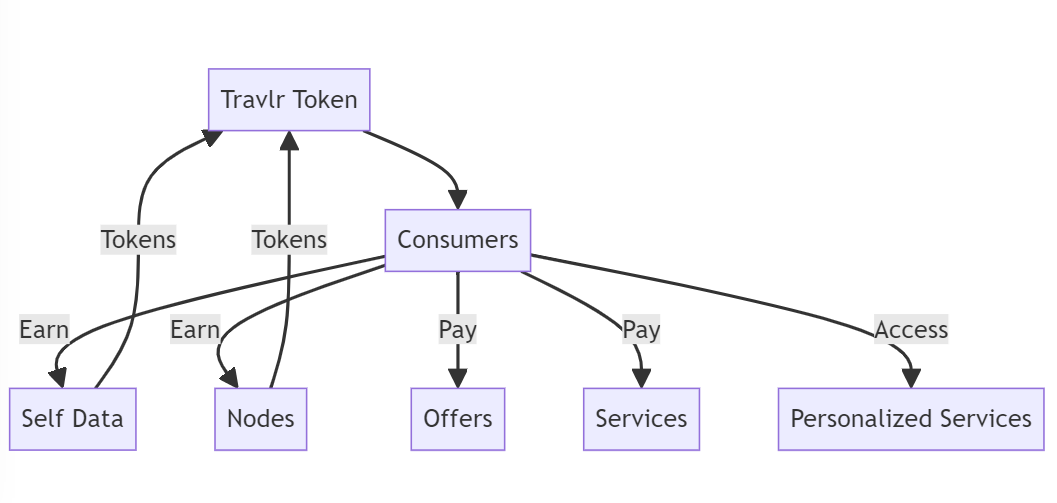
\includegraphics[width=0.7\linewidth]{travlr_diagram_2.png}
    \caption{Consumer utility}
    \label{fig:enter-label}
\end{figure}
Consumers earn Travlr tokens by actively participating in the ecosystem. Key activities that reward tokens include:
\begin{itemize}
    \item \textbf{Self Data}: Users can earn tokens by providing and sharing their personal data. This incentivizes users to contribute valuable data, which enhances the overall data pool and enables better personalization of services.
    \item \textbf{Nodes}: Consumers can run nodes within the Travlr ID network, contributing to the network's decentralization and robustness. Node operators are rewarded with Travlr tokens for their participation and support.
\end{itemize}

\paragraph{Paying with Tokens}

Consumers can use Travlr tokens to access a variety of services within the ecosystem. This includes:
\begin{itemize}
    \item \textbf{Offers}: Tokens can be used to unlock special offers and discounts from participating service providers, enhancing the value proposition for users.
    \item \textbf{Services}: Consumers can pay for personalized travel services and experiences using Travlr tokens, streamlining transactions and ensuring a seamless user experience.

\end{itemize}

\paragraph{Accessing Services}

The use of Travlr tokens facilitates access to personalized services and exclusive offers. This utility ensures that consumers receive tangible benefits from their participation in the ecosystem, driving continued engagement and loyalty.

\subsubsection{Service Providers}

\paragraph{Earning Tokens}
\begin{figure}
    \centering
    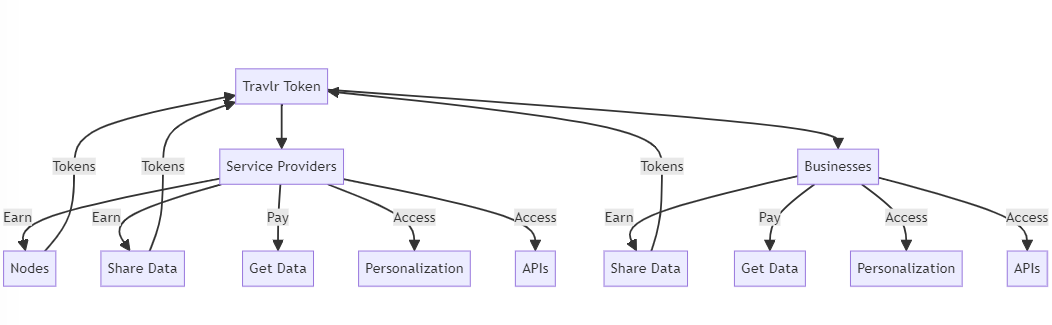
\includegraphics[width=0.8\linewidth]{travlr_diagram_3.png}
    \caption{Service provider \& Business utlity}
    \label{fig:enter-label}
\end{figure}
Service providers earn Travlr tokens through several key activities:
\begin{itemize}
    \item \textbf{Nodes}: Similar to consumers, service providers can operate nodes within the network, earning tokens as a reward for their contribution to the network's infrastructure.
    \item \textbf{Share Data}: Service providers are incentivized to share data with the Travlr ID ecosystem. By contributing valuable data, providers help enhance the overall data quality and utility, benefiting all participants.
\end{itemize}

\paragraph{Paying with Tokens}

Service providers use Travlr tokens to access necessary data and services within the ecosystem. They pay tokens to access consumer data, which they can use to personalize services and improve customer experiences.

\paragraph{Accessing APIs and Personalization}

Service providers utilize Travlr tokens to access APIs that enable seamless integration with the Travlr ID platform. This access facilitates the personalization of services, allowing providers to offer tailored experiences that meet individual consumer needs.

\subsubsection{Businesses}

\paragraph{Earning Tokens}

Businesses earn Travlr tokens by sharing data and contributing to the ecosystem's growth. By participating in the network, businesses enhance the data pool and benefit from the insights generated.

\paragraph{Paying with Tokens}

Businesses utilize Travlr tokens to gain access to consumer data and APIs, which are essential for personalizing services and enhancing operational efficiency. This access drives innovation and competitiveness in the market.

\paragraph{Accessing APIs and Personalization}

Similar to service providers, businesses use Travlr tokens to access APIs that integrate their services with the Travlr ID platform. This integration ensures that businesses can deliver highly personalized services, driving customer satisfaction and loyalty.

\subsection{Ecosystem Dynamics}
\begin{figure}
    \centering
    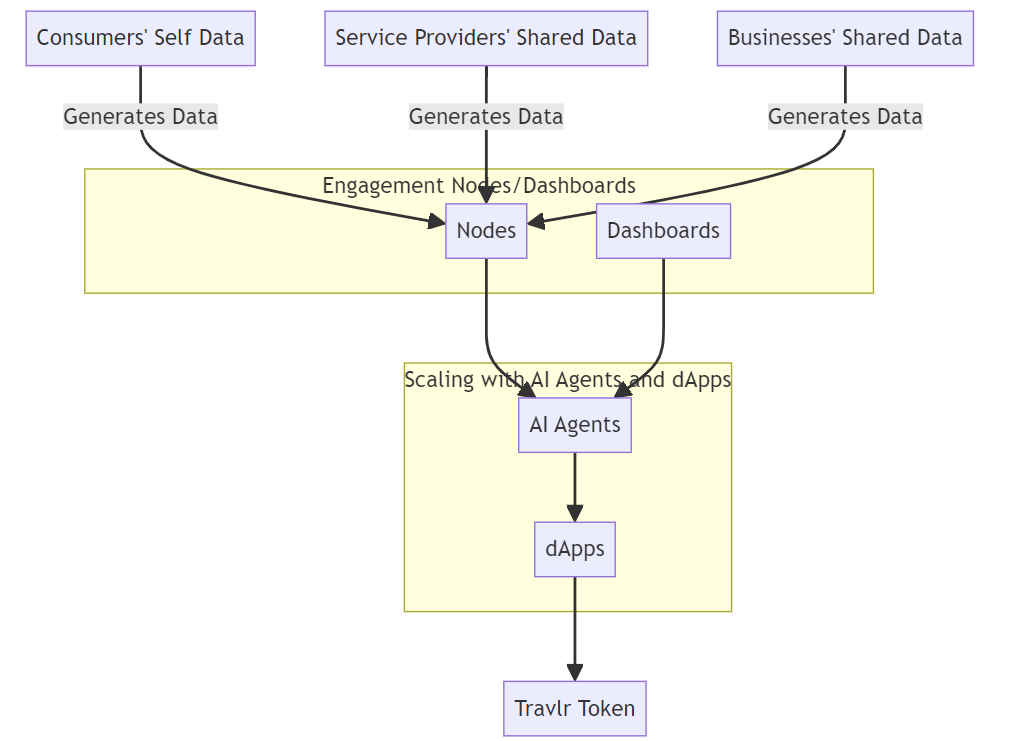
\includegraphics[width=0.8\linewidth]{travlr_diagram_1.png}
    \caption{Ecosystem dynamics}
    \label{fig:enter-label}
\end{figure}
The Travlr token ecosystem is designed to promote a virtuous cycle of data generation, sharing, and utilization. The following key dynamics ensure the ecosystem's sustainability and growth:

\subsubsection{Data Generation and Sharing}

\begin{itemize}
    \item \textbf{Traveler Generates Data}: Travelers generate valuable data as they interact with the Travlr ID ecosystem. This data is securely stored and managed, ensuring user privacy and control.
    \item \textbf{Engagement Nodes/Dashboards}: Nodes and dashboards within the ecosystem facilitate the engagement of users and service providers, ensuring that data is effectively shared and utilized.
\end{itemize}

\subsubsection{Scaling with AI Agents and dApps}

The integration of AI agents and decentralized applications (dApps) within the Travlr ID ecosystem enhances the scalability and functionality of the platform. AI agents analyze data and provide insights, while dApps offer additional services and applications that enhance the user experience.

\subsection{Summary}

The Travlr token is a fundamental component of the Travlr ID ecosystem, providing essential incentives and facilitating transactions that drive engagement and growth. By rewarding data sharing and participation, the token ensures a rich and dynamic data pool, which enhances the overall utility and value of the platform. 

The integration of AI agents and dApps further scales the ecosystem, delivering a seamless and personalized travel experience for all stakeholders. Through its innovative token utility model, Travlr ID is poised to revolutionize the travel industry, offering a future where data management is efficient, secure, and user-centric.

\newpage

\section{Business Model}

The advent of Travlr ID signifies a paradigm shift in the travel industry's approach to data management. At its core, Travlr ID integrates blockchain technology with artificial intelligence to create a Decentralized Physical Infrastructure Network (DePIN). This innovative solution addresses the multifaceted challenges of travel data management by providing consumers with a secure digital vault for their data, and service providers with streamlined, efficient access to this data. The result is a reduction in redundancy and a substantial improvement in service personalization. This whitepaper delves into the intricate technology underpinning Travlr ID, its practical implementation, the myriad benefits it offers, and its potential for future scalability. Through a forward-thinking lens, Travlr ID envisions a transformed travel industry where data management is not only secure and efficient but also fundamentally respectful of user privacy.

\subsection{Core Components}

\subsubsection{Enterprise Console}

\paragraph{Revenue Generation}

The Enterprise Console serves as the primary interface for businesses engaging with the Travlr ID ecosystem. It is a pivotal component for revenue generation, enabling monetization through data access fees and service charges. By providing a seamless interface, businesses can efficiently manage their interactions with the Travlr ID network, ensuring a steady revenue stream.

\paragraph{Travlr ID: Secure Data Management}

At the heart of the Enterprise Console is Travlr ID, which guarantees the secure storage and permissioned sharing of personal data. This feature is crucial for maintaining user trust and ensuring compliance with data protection regulations. Businesses can access this permissioned data to offer highly personalized travel experiences, thereby enhancing customer satisfaction and fostering loyalty.

\paragraph{Permissioned Data and Personalization}

The ability to access permissioned data allows businesses to tailor their services to individual traveler preferences. This level of personalization not only improves the travel experience for consumers but also provides businesses with valuable insights into customer behavior and preferences, driving innovation and competitiveness in the market.

\subsubsection{Travlr ID Mobile App}

\paragraph{Distribution and User Engagement}

The Travlr ID Mobile App acts as the primary touchpoint for consumers within the Travlr ID ecosystem. It is designed to empower users to manage their Travlr ID and interact seamlessly with various service providers. Through this app, users can securely store, manage, and delegate access to their personal data, ensuring that they maintain control over their information.

\paragraph{Personalized Travel Experiences}

The mobile app enables users to access personalized travel services, facilitated by the secure sharing of their data with trusted partners. This personalization is not limited to service recommendations but extends to real-time adjustments and enhancements based on user preferences and behavior, thereby creating a dynamic and responsive travel experience.

\subsection{Service Provider Dashboard}

\paragraph{Efficient Data Access}

The Service Provider Dashboard is a critical tool for service providers, offering efficient access to necessary data. This component reduces redundancy by streamlining data retrieval processes, which in turn minimizes operational overhead. By having real-time access to up-to-date traveler information, service providers can optimize their services and improve operational efficiency.

\paragraph{Enhanced Personalization Capabilities}

Access to detailed traveler data allows service providers to offer highly personalized services. By leveraging data insights, providers can anticipate traveler needs and preferences, delivering a superior and customized service experience. This capability not only enhances customer satisfaction but also fosters a competitive edge in the market.

\begin{figure}[h]
    \centering
    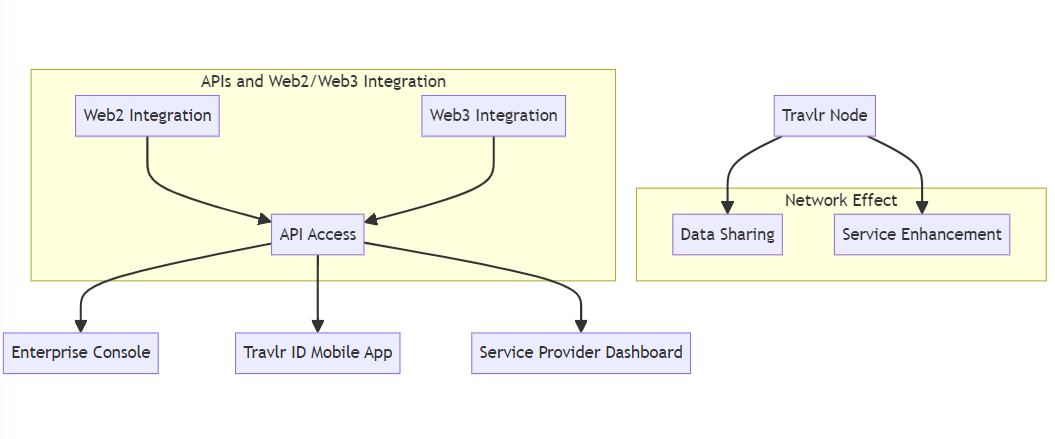
\includegraphics[width=0.8\linewidth]{travlr_diagram_4.png}
    \caption{Business Model}
    \label{fig:enter-label}
\end{figure}

\subsection{Travlr Node}

\paragraph{Token Utility}

The Travlr Node is the central hub of the decentralized network, facilitating various token-based transactions and utility functions. This includes staking and yield generation, which incentivizes user participation and data sharing. The integration of a token-based economy ensures the sustainability and growth of the Travlr ID ecosystem.

\paragraph{Staking and Yield Generation}

Users can engage in staking and yield generation through the Travlr Node, which offers financial incentives for participation in the network. This not only encourages widespread adoption but also enhances the overall security and robustness of the network by ensuring active user involvement.

\paragraph{Transactions and AI Agents}

The integration of AI agents within the Travlr Node enhances the processing and analysis of data. These AI agents are designed to perform a range of tasks, from simple data transactions to complex predictive analytics. This intelligent processing leads to smarter, more efficient operations and enables the delivery of highly personalized travel experiences.

\subsection{Network Effect}

The Travlr ID ecosystem is designed to capitalize on network effects, wherein the value of the network amplifies as more participants—both consumers and service providers—join and contribute data. This collaborative approach ensures a continuously improving and scalable system that benefits all stakeholders. As the network grows, the data pool becomes richer, enabling more accurate personalization and better service offerings.

\subsection{APIs and Web2/Web3 Integration}

Travlr ID bridges traditional web technologies (Web2) with the decentralized future (Web3), providing robust APIs that enable seamless integration and interoperability. This dual compatibility ensures a smooth transition for businesses adopting the platform, facilitating widespread adoption and integration. By offering APIs that cater to both Web2 and Web3 environments, Travlr ID ensures that existing systems can easily integrate with its decentralized infrastructure, thereby reducing the barriers to entry and promoting adoption.

\subsection{Summary}

Travlr ID is poised to transform the travel industry by introducing a secure, efficient, and privacy-respecting data management system. Through its innovative use of blockchain and AI, Travlr ID offers a future where personalized travel experiences are the norm, and data management is both secure and efficient. 

The Travlr ID business model, supported by a robust DePIN and intelligent AI agents, promises to revolutionize the way travel data is managed and utilized. This transformation paves the way for a smarter, more connected travel ecosystem, where data-driven insights lead to enhanced traveler experiences and operational efficiencies. With its forward-thinking approach and robust technological foundation, Travlr ID is set to redefine the future of travel data management.

\newpage

\section{Conclusion}

Data circulation is the lifeblood of the travel industry: a complex web of informational exchanges occurring between multiple different entities. However, the current state of data management in the sector is far from ideal, caught in a quagmire comprising fragmented data silos, cumbersome verification processes, privacy issues, and potential vulnerabilities to data breaches. 

Within this scenario, Travlr ID emerges as a leading solution. By employing the power of blockchain technology, decentralization, and state-of-the-art data security protocols, Travlr ID places the control of personal information firmly into the consumer's hands while simultaneously streamlining functionalities for service providers. 

The architecture of Travlr ID has been specially designed to address the unique demands and challenges of the travel industry. Digital vaults for consumers and service providers promote seamless data exchange, while the on-prem nodes managed by service providers ensure data control \& effective utilization. Furthermore, this architecture paves the path towards adopting emerging technologies like decentralized AI, thereby amplifying personalisation and operational efficiency. 

A key aspect of the Travlr ID solution is its focus on privacy and regulatory aspects. Respect for user data and strict adherence to international data protection norms are woven into its fabric. Advanced practices such as Zero-knowledge proofs keep customer information secure without diminishing the validity of transactions. 

In terms of scalability and future growth, Travlr ID holds tremendous promise. Its inherent design to function across multiple blockchain platforms and commitment to maintaining reasonable transaction and storage costs position it well for wide-scale adoption and expansion. 

The profound benefits that Travlr ID stands to bring to consumers and service providers, as depicted in the use cases, underscore how this unique approach revolutionizes the travel experience: simplifying processes, enhancing personalisation, and maintaining security at the core. 

As we stand at the precipice of a new era in travel data management, Travlr ID is geared up to lead this exciting journey, transforming the way we approach travel planning today and setting the pace for the industry's future. This intricate blend of technology, privacy, and service personalisation sets Travlr ID apart, marrying the power of blockchain with the dynamic world of travel, thus redefining the realm of possibilities within the travel industry. 

We believe that Travlr ID represents a significant leap forward, heralding a new chapter in the travel industry that is characterized by seamless data exchanges, enhanced privacy control, and streamlined, personalized experiences. Guided by a vision of a decentralized and privacy-respecting travel industry and powered by cutting-edge technology, Travlr ID is set to navigate the industry towards a revolutionary transformation.

\end{document}